\chapter{Web aplikacija}

Sustav kontrole i evidencije pristupa viđen s visoke razine sastoji se od tri cjeline:
\begin{itemize}
    \item Infrastruktura
    \item Pozadinska aplikacija
    \item Grafičko sučelje
\end{itemize}

U ovom poglavlju sve tri cjeline će biti opisane i razrađene.

\section{Infrastruktura}

Infrastruktura je sačinjena od servera, čvorova, usmjerivača i sl.
Također, infrastrukturu čini operacijski sustav, vatrozid, i ostali softver\cite{ibm-infrastructure}.
Po tom pitanju danas se ništa značajno nije promijenilo, samo su fizičke komponente skrivene u "oblaku" (eng. \textit{cloud}).
Rad zahtjeva vrlo jednostavnu infrastrukturu pa je oblak prikladno rješenje jer ne zahtjeva vlastoručnu konfiguraciju i održavanje fizičkih komponenti.

\begin{figure}[h!]
    \centering
    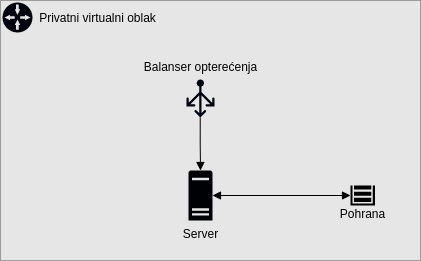
\includegraphics[scale=0.7]{images/infrastructure}
    \caption{Fizičke komponente infrastrukture}
    \label{fig:physical-infrastructure}
\end{figure}

Na slici~\ref{fig:physical-infrastructure} nalazu se sve komponente kreirane kod pružatelja usluge oblaka (DigitalOcean).
Privatni virtualni oblak ima mnoštvo značajki, ali u ovom slučaju se koristi samo za logičko grupiranje komponenti.
Balanser opterećenja (eng. \textit{load balancer}) služi kao \textit{proxy} do glavnog servera i moguće je povezati domenu na njega.
Server ima vlastitu sekundarnu pohranu na kojoj se nalazi operacijski sustav i potrebni alati ali i vanjsku pohranu na kojoj se nalaze aplikacijski podaci.

Vanjska pohrana i balanser opterećenja izgledaju, na prvi pogled, nepotrebni.
U scenariju kad se glavni server nepovratno sruši vrlo je lako kreirati novi i nastaviti s normalnim radom.
Krajnji korisnik osjeti kratki prekid usluge, a ne potpuni gubitak usluge i podataka.
U slučaju samo jednog servera (bez vanjske pohrane i balansera opterećenja) podaci i IP adresa se trajno gube što predstavlja veliku
neugodnost krajnjem korisniku.
